\documentclass[tikz]{standalone}
\usepackage{tikz}
\pagestyle{empty}

\newcommand{\dvec}[1]{\textbf{\overrightarrow{#1}}}

\begin{document}
    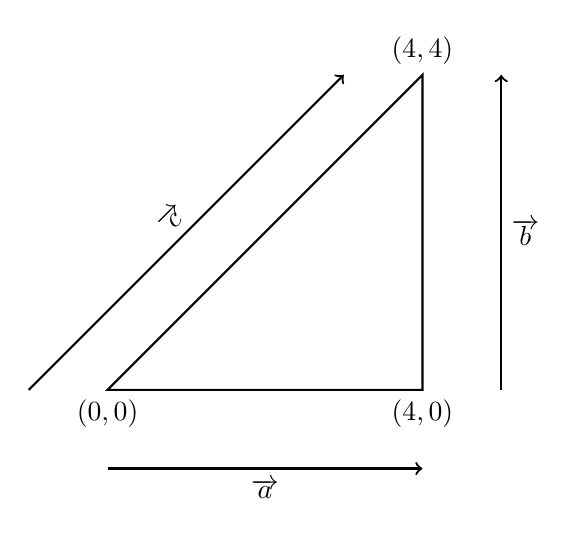
\begin{tikzpicture}
        \draw [thick]
        (0,0) node[anchor=north]{$(0,0)$} --
        (4,0) node[anchor=north]{$(4,0)$} --
        (4,4) node[anchor=south]{$(4,4)$} -- cycle;
        \draw [->, thick] (0,-1) -- node[anchor=north]{$\dvec{a}$} (4,-1);
        \draw [->, thick] (5,0)  -- node[anchor=west]{$\dvec{b}$} (5,4);
        \draw [->, thick] (-1,0) -- node[anchor=south,rotate=45]{$\dvec{c}$} (3,4);
    \end{tikzpicture}
\end{document}
